% !TEX root = ./architecture.tex

\KOMAoption{headsepline}{true}

\chead[]{Explainable Similarity Detector}

\ifoot{AMOS WS 2021/2022 - Pr. 6}
\cfoot[]{\pagemark}
\ofoot{\todayGer}

\section{Laufzeit Komponenten}

% An overview diagram of runtime components (one page)

Überblick über die Laufzeit Komponenten

\vspace*{\fill}

\begin{figure}[ht]
    \centering
    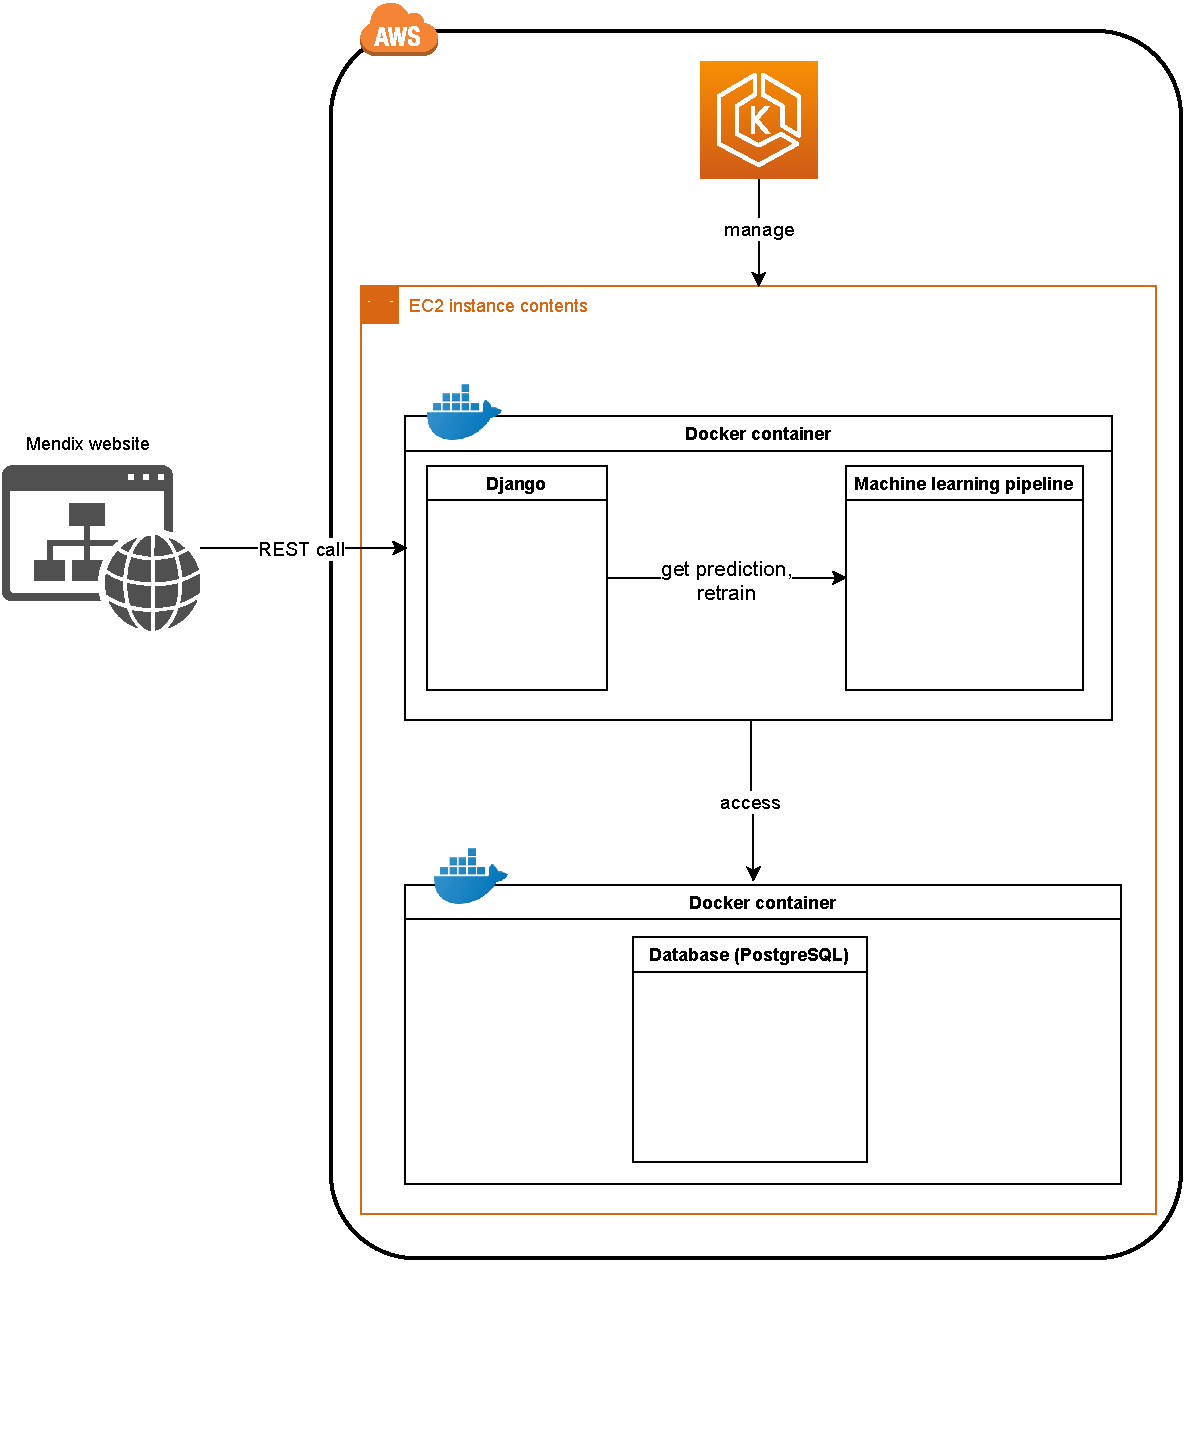
\includegraphics[%
        width=0.96\textwidth,
        clip, 
        trim=0cm 2.7cm 0cm 0cm % trim=left botm right top
    ]{../runtime-components/runtime-components}
    \caption{Laufzeit Komponenten}
    \label{fig:runtime-components}
\end{figure}

\vspace*{\fill}

\newpage

\section{Code Komponenten}

% An overview diagram of code components (one page)

Überblick über die Code Komponenten

\vspace*{\fill}

\begin{figure}[ht]
    \centering
    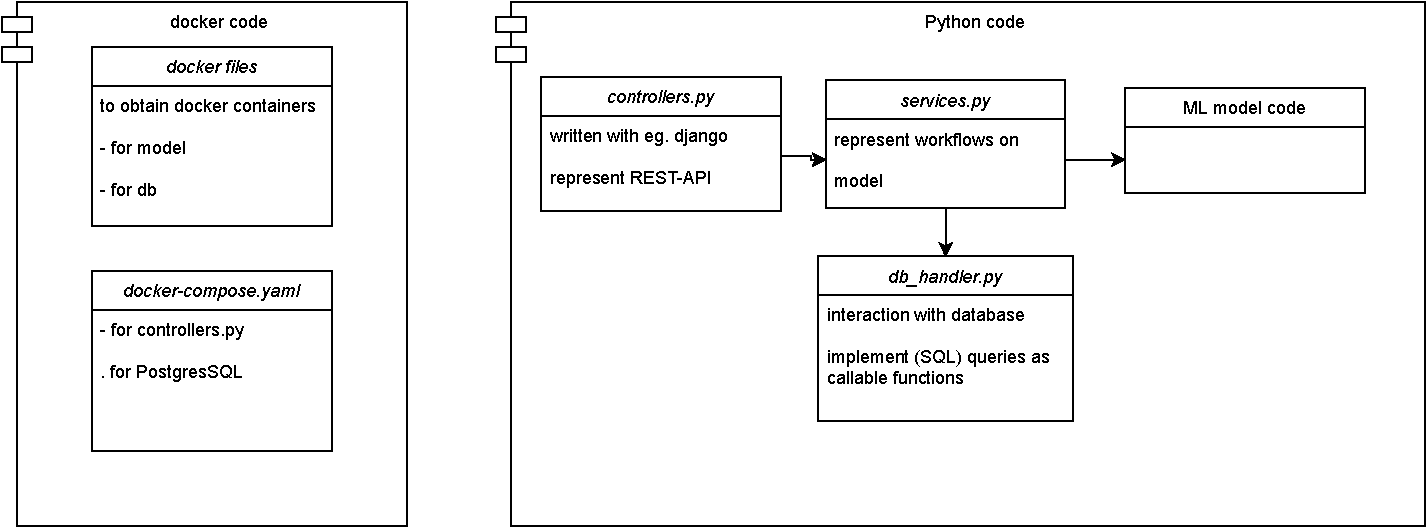
\includegraphics[%
        width=0.96\textwidth,
        clip, 
    ]{../code-components/code-components}
    \caption{Code Komponenten}
    \label{fig:code-components}
\end{figure}

\vspace*{\fill}

\newpage

\section{Technologie-Stack}

% A summary of the underlying technology stack (one page)

Zusammenfassung des zugrunde liegenden Technologie-Stacks

\newpage

\section{Textuelle Erklärung}

% A textual explanation of the diagrams and choices (one page)

Textuelle Erläuterung der Diagramme und Auswahlmöglichkeiten

